\documentclass[../thesis.tex]{subfiles}

\begin{document}

Google Translate là một dịch vụ dịch thuật được phát triển bởi Google hỗ trợ trên 100 ngôn ngữ. Số liệu thống kê vào tháng 05 năm 2013 cho thấy, Google Translate phục vụ dịch thuật cho hơn 200 triệu người mỗi ngày.

Google Cloud Translation API là một API thuộc Cloud Machine Learning API. Cloud Translation API cung cấp một giao diện lập trình ứng dụng đơn giản để lập trình viên có thể tích hợp tính năng phiên dịch (Translation) của Google vào website hoặc ứng dụng của họ. Với tính tương thích cao, các website và ứng dụng tích hợp Google Translation API hoạt động rất hiệu quả trong việc phiên dịch từ một ngôn ngữ sang một ngôn ngữ khác (Ví dụ: từ tiếng Anh sang tiếng Việt). Ngoài ra, tính năng nhận diện ngôn ngữ cũng hoạt động khá hiệu quả khi ngôn ngữ gốc chưa được xác định.

\section{Đăng ký sử dụng Google Cloud Platform}
Ta sử dụng tài khoản Google để truy cập đến các dịch vụ của Google Cloud Platform. Để nhận \$300 credit dùng thử trong 1 năm từ Google, ta truy cập vào link:
\begin{lstlisting}[numbers=none, frame=none,xleftmargin=0cm]
https://console.cloud.google.com/freetrial
\end{lstlisting}
và điền đầy đủ các thông tin mà Google yêu cầu, bao gồm cả thông tin thẻ tín dụng.

\section{Tạo một project trên Google API Console}
\begin{enumerate}
	\item Truy cập vào Google Cloud Platform Console.
	\item Tạo một project tên là ``translation'' (Hình \ref{Tạo một project trên Google Cloud Platform}).
	\begin{figure}
		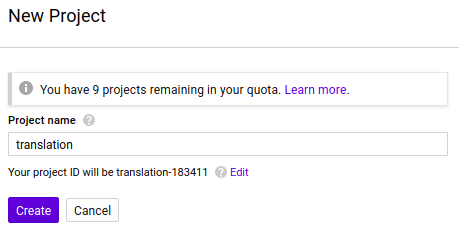
\includegraphics[width=\textwidth, keepaspectratio]{create-project.png}
		\caption{Tạo một project trên Google Cloud Platform}
		\label{Tạo một project trên Google Cloud Platform}
	\end{figure}
\end{enumerate}

\section{Kích hoạt Google Cloud Translation API}
\begin{enumerate}
	\item Từ thanh tìm kiếm, nhập từ khoá ``Google Cloud Translation API''.
	\item Nhấp vào nút Enable để kích hoạt dịch vụ Translation.
	% TODO: Chèn hình vào đây và ref lên trên
\end{enumerate}

\section{Lấy API Key}
\begin{enumerate}
	\item Từ Google Cloud Platform Console menu, vào APIs and services > Credentials.
	\item Tạo một API key.
	% TODO: Chèn hình vào đây và ref lên trên
\end{enumerate}

\section{Xác minh quyền truy cập đến Google Translation API}

\section{Tạo một project trên Eclipse}
\begin{enumerate}
	\item Cài đặt gói M2Eclipse.

	\item Vào File > New > Other\ldots > Maven > Maven Project. (Hình \ref{Tạo một project Maven trên Eclipse} và \ref{Thiết lập Archetype Parameters})
	\begin{figure}
		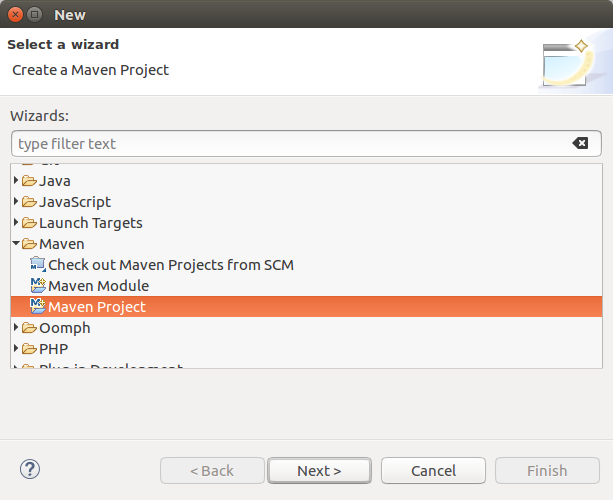
\includegraphics[width=\textwidth, keepaspectratio]{create-maven-project-1.png}
		\caption{Tạo một project Maven trên Eclipse}
		\label{Tạo một project Maven trên Eclipse}
	\end{figure}
	\begin{figure}
		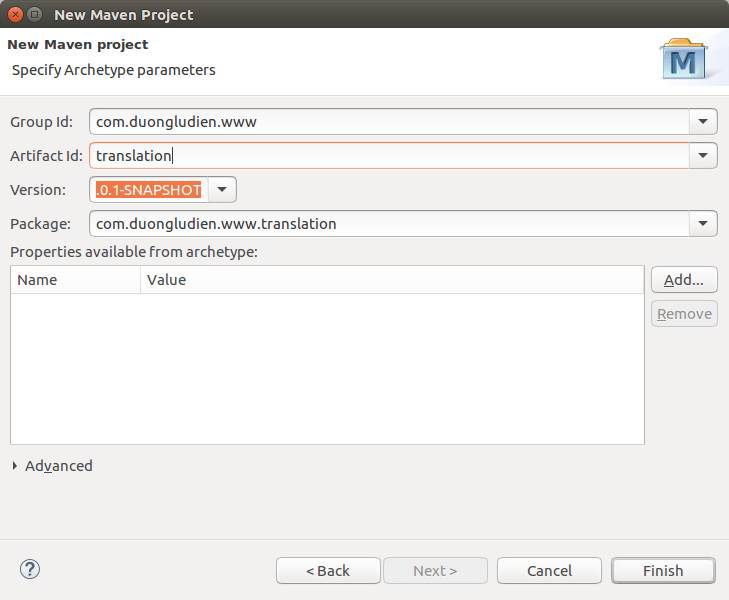
\includegraphics[width=\textwidth, keepaspectratio]{create-maven-project-2.png}
		\caption{Thiết lập Archetype Parameters}
		\label{Thiết lập Archetype Parameters}
	\end{figure}
	
	\item Mở file cấu hình Maven pom.xml vào thêm vào mục Dependencies\footnote{https://developers.google.com/api-client-library/java/apis/translate/v2} (Hình \ref{Thêm Dependencies}).
	\begin{itemize}
		\item Group Id: com.google.apis
		\item Artifact Id: google-api-services-translate
		\item Version: v2-rev51-1.23.0
	\end{itemize}
	\begin{figure}
		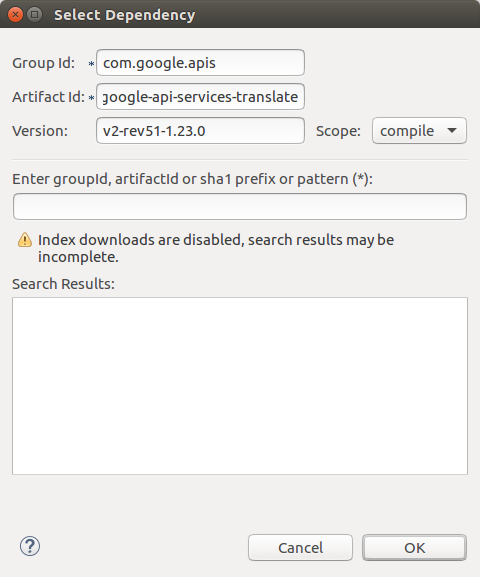
\includegraphics[width=\textwidth, keepaspectratio]{create-maven-project-3.png}
		\caption{Thêm Dependencies}
		\label{Thêm Dependencies}
	\end{figure}
\end{enumerate}
\end{document}